\documentclass{standalone}
\usepackage{tikz}
\usepackage{ctex,siunitx}
\setCJKmainfont{Noto Serif CJK SC}
\usepackage{tkz-euclide}
\usepackage{amsmath}
\usetikzlibrary{patterns, calc,3d}
\usetikzlibrary {decorations.pathmorphing,decorations.pathreplacing,decorations.shapes,}
\tikzset{label style/.append style={font=\small}}
\begin{document}
\small
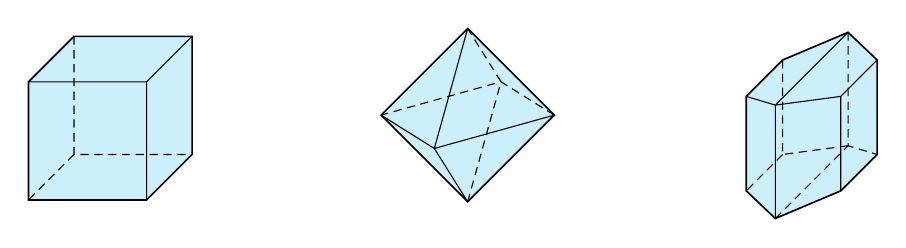
\begin{tikzpicture}[>=latex,scale=1.0]
  \begin{scope}[scale=1.5]
  \draw[fill=cyan!20,semithick](1,0,0)--(1,1,0)--(0,1,0)--(0,1,1)--(0,0,1)--(1,0,1)--cycle;
  \draw[thin](0,1,1)--(1,1,1)--(1,1,0)(1,1,1)--(1,0,1);
  \draw[thin,densely dashed](0,1,0)--(0,0,0)--(1,0,0)(0,0,0)--(0,0,1);
  \end{scope}
  \begin{scope}[xshift=5cm,yshift=5mm,scale=1.1]
    \draw[fill=cyan!20,semithick](0,1,0)--(-1,0,0)--(0,-1,0)--(1,0,0)--cycle;
  \draw[thin](1,0,0)--(0,0,1)--(-1,0,0)(0,-1,0)--(0,0,1)--(0,1,0);
  \draw[thin,densely dashed](1,0,0)--(0,0,-1)--(-1,0,0)(0,-1,0)--(0,0,-1)--(0,1,0);
  \end{scope}
  \begin{scope}[xshift=9cm,scale=1.2]
    \draw[fill=cyan!20,semithick](1,0,0)--(1,1,0)--(0.5,1.1,-0.5)--(0,1,0)--(0,1,1)--(0,0,1)--(0.5,-0.1,1.5)--(1,0,1)--cycle;
    \draw[thin](0,1,1)--(0.5,1.1,1.5)--(1,1,1)--(1,1,0)(1,1,1)--(1,0,1);
    \draw[thin](0.5,-0.1,1.5)--(0.5,1.1,1.5)--(0.5,1.1,-0.5);
    \draw[thin,densely dashed](0.5,1.1,-0.5)--(0.5,-0.1,-0.5)--(1,0,0)(0,1,0)--(0,0,0)--(0.5,-0.1,-0.5)(0,0,0)--(0,0,1)(0.5,-0.1,1.5)--(0.5,-0.1,-0.5);
  \end{scope}
\end{tikzpicture}
\end{document}